\begin{enumerate}[label=\thesubsection.\arabic*,ref=\thesubsection.\theenumi]
    \item Find the shortest distance between the lines whose vector equations are
    \begin{align}
        \vec{x} = \myvec{1\\2\\3} + \lambda_1\myvec{1\\-3\\2}
    \end{align}
    and
    \begin{align}
        \vec{x} = \myvec{4\\5\\6} + \lambda_2\myvec{2\\3\\1}
    \end{align}
    \solution
		    For this problem,
    \begin{align}
        \vec{x} = \vec{x_2} - \vec{x_1} = \myvec{3\\3\\3} \\
        \vec{M} = \myvec{\vec{m_1} & \vec{m_2}} = \myvec{1&2\\-3&3\\2&1} 
    \end{align}
    Thus,
    \begin{align}
        \vec{M}^\top\vec{M} = \myvec{1&-3&2\\2&3&1}\myvec{1&2\\-3&3\\2&1} = \myvec{14&-5\\-5&14} \\
        \vec{MM}^\top = \myvec{1&2\\-3&3\\2&1}\myvec{1&-3&2\\2&3&1} = \myvec{5&3&4\\3&18&-3\\4&-3&5}
    \end{align}
    We perform the eigendecompositions for each matrix and bring them into the form
    \begin{align}
        \vec{MM}^\top &= \vec{P_1D_1P_1}^\top \label{eq:chapters/12/11/2/16/svd/decomp-1} \\
        \vec{M}^\top\vec{M} &= \vec{P_2D_2P_2}^\top \label{eq:chapters/12/11/2/16/svd/decomp-2}
    \end{align}
    \begin{enumerate}
        \item For $\vec{MM}^\top$, the characteristic polynomial is
        \begin{align}
		\text{char}{\vec{MM}^\top} &= \mydet{x-5&-3&-4\\-3&x-18&3\\-4&3&x-5} \\
                                      &= x\brak{x-9}\brak{x-19}
                                      \label{eq:chapters/12/11/2/16/svd/char-2}
        \end{align}
        Thus, the eigenvalues are given by
        \begin{align}
            \lambda_1 = 19,\ \lambda_2 = 9,\ \lambda_3 = 0
        \end{align}
        For $\lambda_1$, the augmented matrix formed from the 
        eigenvalue-eigenvector equation is
        \begin{align}
            &\myvec{-14&3&4&0\\3&-1&-3&0\\4&-3&-14&0} \nonumber \\
            &\xleftrightarrow[]{R_1 \leftarrow \frac{R_1+R_3}{-10}} \myvec{1&0&1&0\\3&-1&-3&0\\4&-3&-14&0} \\
            &\xleftrightarrow[]{R_2 \leftarrow -R_2+3R_1} \myvec{1&0&1&0\\0&1&6&0\\4&-3&-14&0} \\
            &\xleftrightarrow[]{R_3 \leftarrow R_3-4R_1} \myvec{1&0&1&0\\0&-1&-6&0\\0&-3&-18&0} \\
            &\xleftrightarrow[]{R_3 \leftarrow R_3-3R_2} \myvec{1&0&1&0\\0&-1&-6&0\\0&0&0&0}
        \end{align}
        Hence, the normalized eigenvector is
        \begin{align}
            \vec{p_1} = \frac{1}{\sqrt{38}}\myvec{-1\\-6\\1}
        \end{align}
        For $\lambda_2$, the augmented matrix formed from the 
        eigenvalue-eigenvector equation is
        \begin{align}
            &\myvec{-4&3&4&0\\3&9&-3&0\\4&3&-4&0} \nonumber \\
            &\xleftrightarrow[]{R_3 \leftarrow R_1+R_3} \myvec{-4&3&4&0\\3&9&-3&0\\0&0&0&0} \\
            &\xleftrightarrow[]{R_2 \leftarrow \frac{4R_2+3R_1}{45}} \myvec{-4&3&4&0\\0&1&0&0\\0&0&0&0} \\
            &\xleftrightarrow[]{R_1 \leftarrow \frac{R_1-3R_2}{-4}} \myvec{1&0&-1&0\\0&1&0&0\\0&0&0&0}
        \end{align}
        Hence, the normalized eigenvector is
        \begin{align}
            \vec{p_2} = \frac{1}{\sqrt{2}}\myvec{1\\0\\1}
        \end{align}
        For $\lambda_3$, the augmented matrix formed from the 
        eigenvalue-eigenvector equation is
        \begin{align}
            &\myvec{5&3&4&0\\3&18&-3&0\\4&-3&5&0} \nonumber \\ 
            &\xleftrightarrow[]{R_1 \leftarrow \frac{R_1+R_3}{9}} \myvec{1&0&1&0\\3&18&-3&0\\4&-3&5&0} \\
            &\xleftrightarrow[]{R_2 \leftarrow R_2-3R_1} \myvec{1&0&1&0\\0&18&-6&0\\4&-3&5&0} \\
            &\xleftrightarrow[]{R_3 \leftarrow R_3-4R_1} \myvec{1&0&1&0\\0&18&-6&0\\0&-3&1&0} \\
            &\xleftrightarrow[]{R_2 \leftarrow \frac{R_2}{6}} \myvec{1&0&1&0\\0&3&-1&0\\0&-3&1&0} \\
            &\xleftrightarrow[]{R_3 \leftarrow R_3+R_2} \myvec{1&0&1&0\\0&3&-1&0\\0&0&0&0}
        \end{align}
        Hence, the normalized eigenvector is
        \begin{align}
            \vec{p_3} = \frac{1}{\sqrt{19}}\myvec{-3\\1\\3}
        \end{align}
        Using \eqref{eq:chapters/12/11/2/16/svd/decomp-1}, we see that
        \begin{align}
            \vec{P_1} = \myvec{-\frac{1}{\sqrt{38}}&\frac{1}{\sqrt{2}}&-\frac{3}{\sqrt{19}}\\-\frac{6}{\sqrt{38}}&0&\frac{1}{\sqrt{19}}\\\frac{1}{\sqrt{38}}&-\frac{1}{\sqrt{2}}&\frac{3}{\sqrt{19}}} \\
            \vec{D_1} = \myvec{19&0&0\\0&9&0\\0&0&0}
            \label{eq:chapters/12/11/2/16/svd/eig-params-1}
        \end{align}
        \item For $\vec{M}^\top\vec{M}$, the characteristic polynomial is
        \begin{align}
		\text{char}{\vec{M}^\top\vec{M}} &= \mydet{x-14&5\\5&x-14} \\
                                      &= \brak{x-9}\brak{x-19}
%                                      \label{eq:chapters/12/11/2/16/svd/char-1}
        \end{align}
        Thus, the eigenvalues are given by
        \begin{align}
            \lambda_1 = 19,\ \lambda_2 = 9
        \end{align}
        For $\lambda_1$, the augmented matrix formed from the 
        eigenvalue-eigenvector equation is
        \begin{align}
            \myvec{-5&-5&0\\-5&-5&0} &\xleftrightarrow[]{R_1 \leftarrow R_1-R_2} \myvec{0&0&0\\-5&-5&0}
        \end{align}
        Hence, the normalized eigenvector is
        \begin{align}
            \vec{p_1} = \frac{1}{\sqrt{2}}\myvec{1\\-1}
        \end{align}
        For $\lambda_2$, the augmented matrix formed from the 
        eigenvalue-eigenvector equation is
        \begin{align}
            \myvec{5&-5&0\\-5&5&0} &\xleftrightarrow[]{R_1 \leftarrow R_1+R_2} \myvec{0&0&0\\5&-5&0}
        \end{align}
        Hence, the normalized eigenvector is
        \begin{align}
            \vec{p_2} = \frac{1}{\sqrt{2}}\myvec{1\\1}
        \end{align}
        Thus, from \eqref{eq:chapters/12/11/2/16/svd/decomp-2},
        \begin{align}
            \vec{P_2} = \myvec{\frac{1}{\sqrt{2}}&-\frac{1}{\sqrt{2}}\\\frac{1}{\sqrt{2}}&\frac{1}{\sqrt{2}}},\ \vec{D_2} = \myvec{9&0\\0&19}
            \label{eq:chapters/12/11/2/16/svd/eig-params-2}
        \end{align}
    \end{enumerate}
    Therefore, from \eqref{eq:chapters/12/11/2/16/svd/M-svd},
    \begin{align}
        \vec{U} &= \vec{P_1} \\ 
        \vec{V} &= \vec{P_2} \\
        \vec{\Sigma} &= \myvec{\sqrt{19}&0\\0&3\\0&0}
        \label{eq:chapters/12/11/2/16/svd/svd-params}
    \end{align}
    and substituting into \eqref{eq:chapters/12/11/2/16/svd/lambda-sol}, we get
    \begin{align}
        \vec{\lambda} = \frac{1}{19}\myvec{10\\28}
    \end{align}
    which agrees with earlier solutions as well.
    \iffalse
    The Python code
    \texttt{codes/svd.py} plots 
    \fi
    See Fig. \ref{fig:chapters/12/11/2/16/svd/svd} depicting the situation.
    \begin{figure}[!ht]
        \centering
        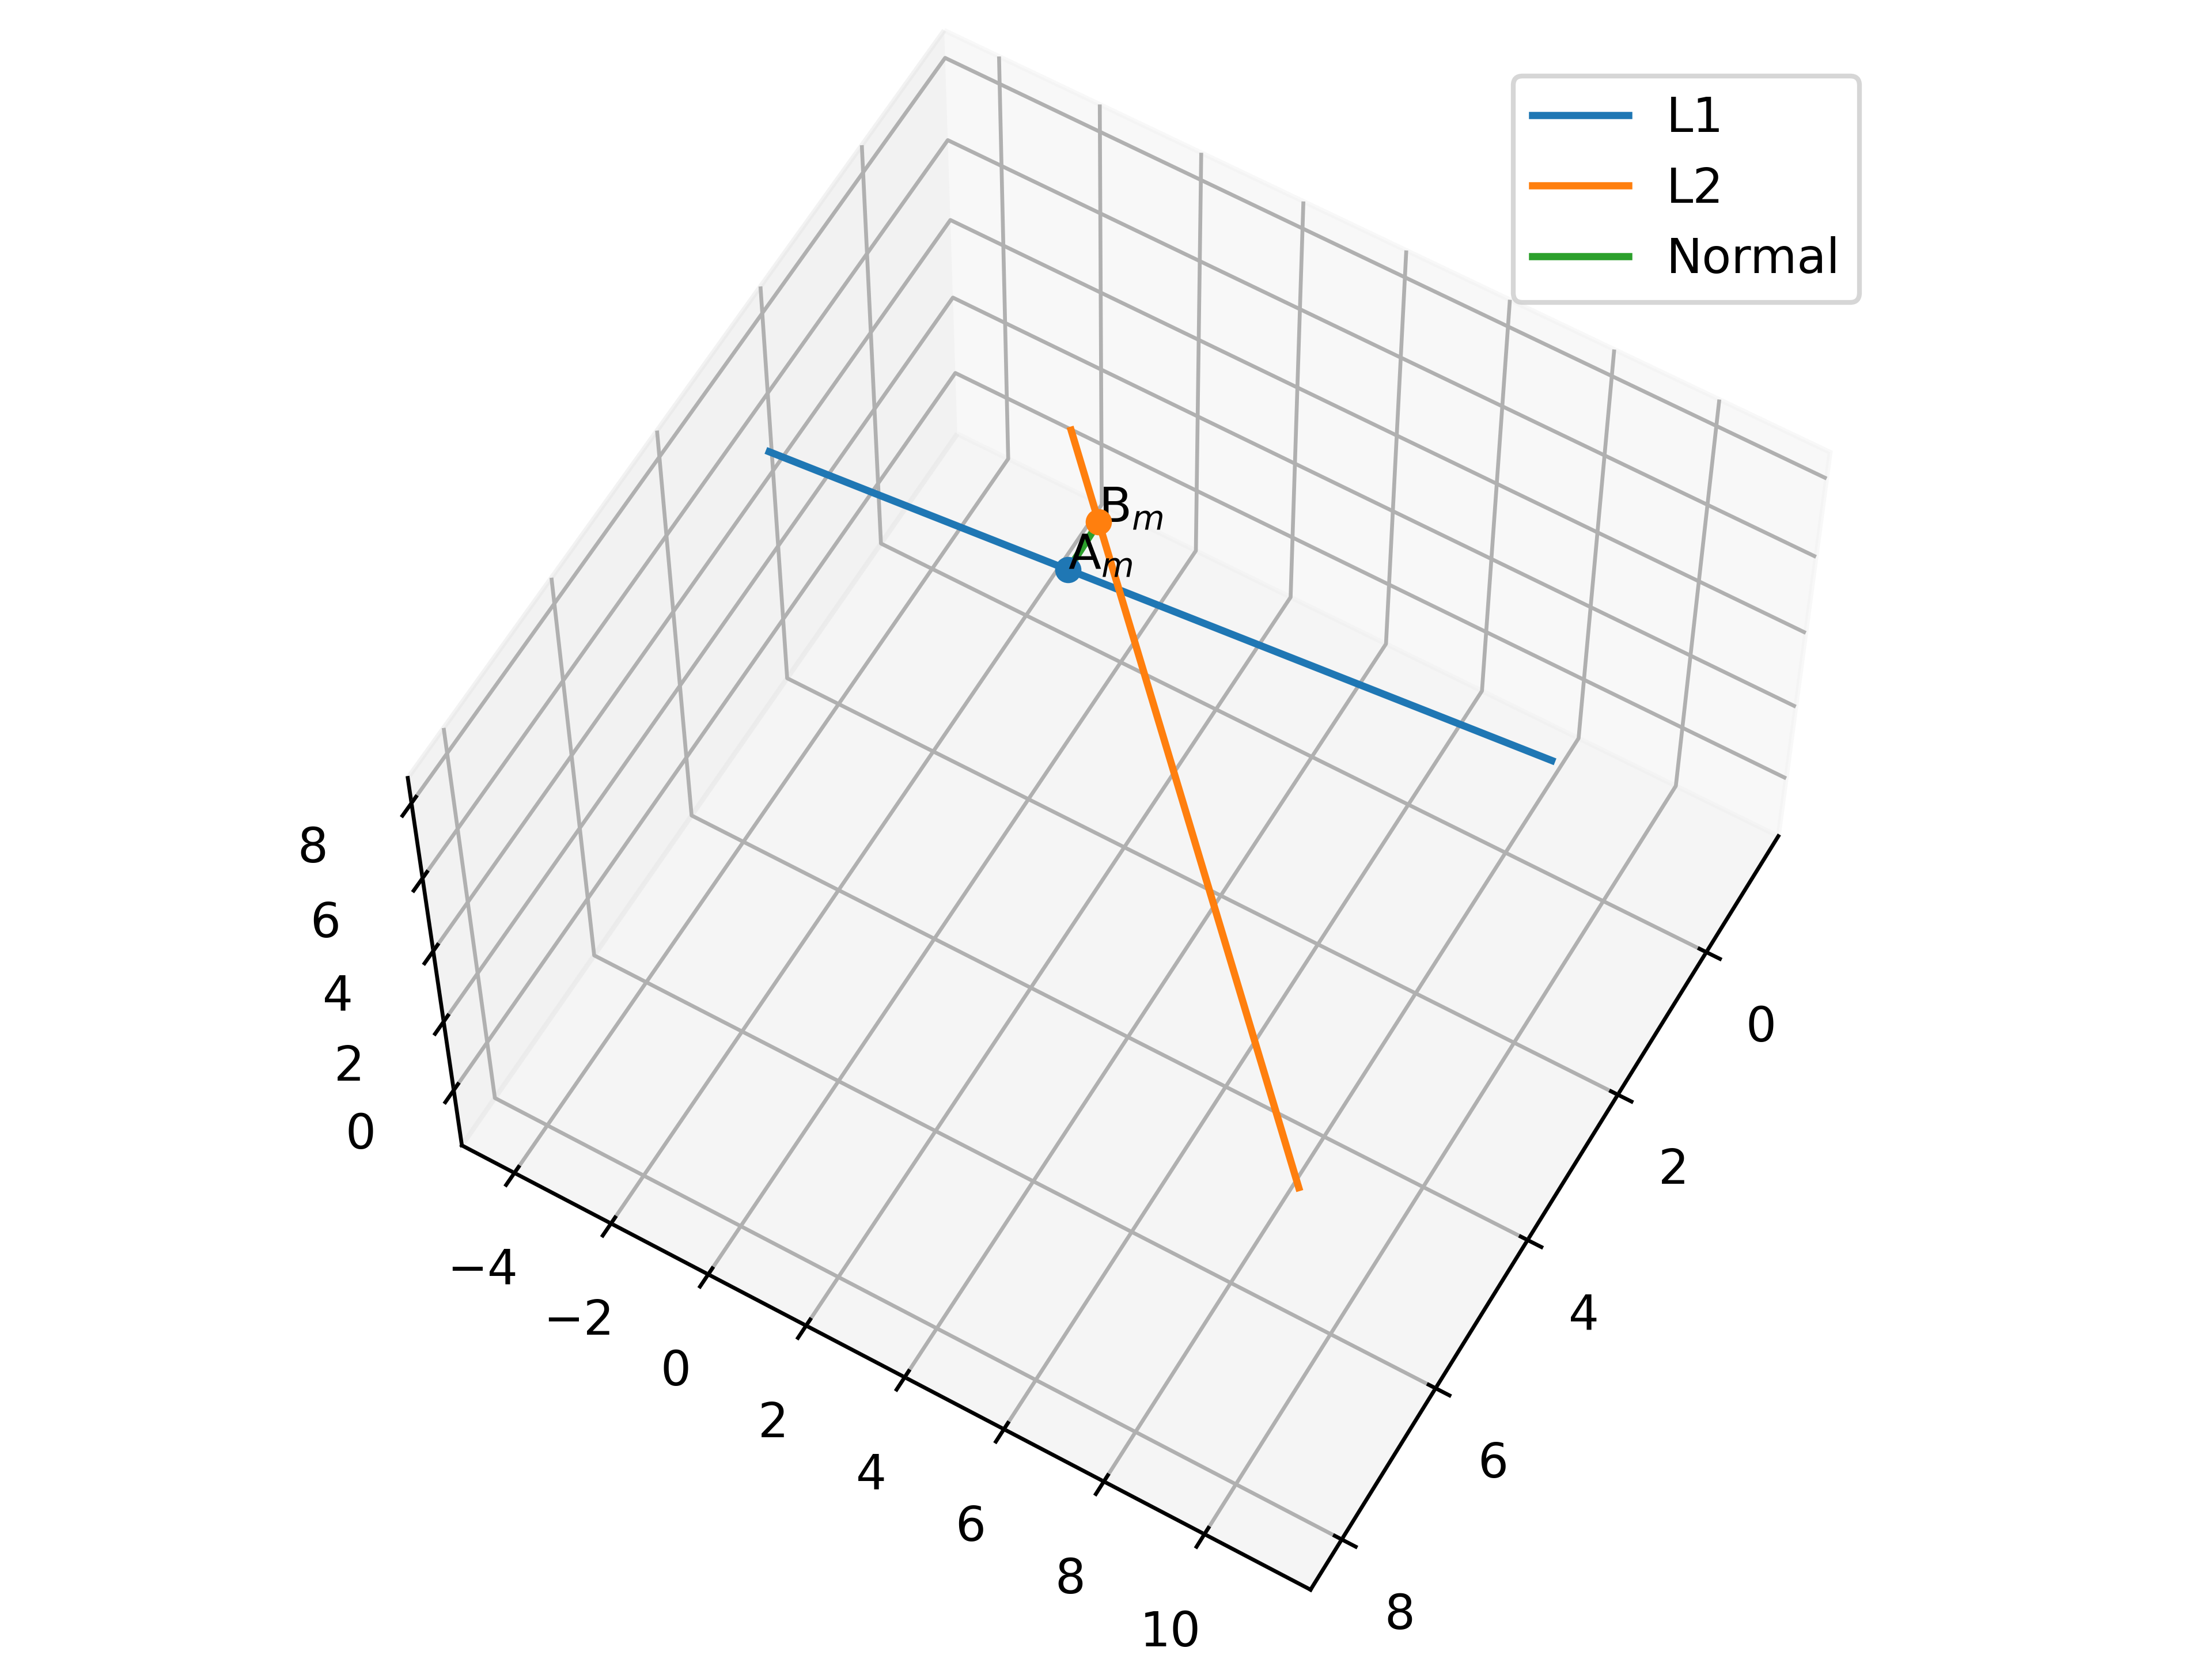
\includegraphics[width=\columnwidth]{chapters/12/11/2/16/svd/figs/skew_svd.png}
        \caption{Finding the shortest distance between two lines using SVD.}
        \label{fig:chapters/12/11/2/16/svd/svd}
    \end{figure}

\item Find the shortest distance between the lines $l_1$ and $l_2$ whose vector equations are 
\begin{align}
	\overrightarrow{r} &= \hat{i}+\hat{j}+\lambda(2\hat{i}-\hat{j}+\hat{k}) \text{ and}
	\\
	\overrightarrow{r} &= 2\hat{i}+\hat{j}-\hat{k}+\mu(3\hat{i}-5\hat{j}+2\hat{k}).
\end{align}
    \solution
		\begin{enumerate}
\item 
To check whether the given lines are skew,
from \eqref{eq:chapters/12/11/2/e11/params}
and 
	    \eqref{eq:chapters/12/11/2/16/lsq/rank},

\begin{align*}
\myvec{2&3&&1\\-1&-5&&0\\1&2&&-1}
\xleftrightarrow[R_3 \leftarrow R_3 - \frac{1}{2}R_1]{R_2 \leftarrow R_2 + \frac{1}{2}R_1}
\myvec{2&3&&1\\[1ex]0&-\frac{7}{2}&&\frac{1}{2}\\[1ex]0&\frac{1}{2}&&-\frac{3}{2}}\\
\xleftrightarrow{R_3 \leftarrow R_3 + 7R_2}
\myvec{2&3&&1\\[1ex]0&-\frac{7}{2}&&\frac{1}{2}\\[1ex]0&0&&-10}
\end{align*}
The rank of the matrix is 3. So the given lines are skew.
\item 
\begin{align}
\vec{M}^\top\vec{M} &= \myvec{2&-1&1\\3&-5&2}\myvec{2&3\\-1&-5\\1&2} \\ 
&= \myvec{6&13\\13&38} \label{eq:chapters/12/11/2/311/svd/MtM}
\end{align}
\begin{align}
\vec{MM}^\top &= \myvec{2&3\\-1&-5\\1&2}\myvec{2&-1&1\\3&-5&2}\\
&= \myvec{13&-17&8\\-17&26&-11\\8&-11&5} \label{eq:chapters/12/11/2/311/svd/MMt}
\end{align}
The characteristic polynomial of the matrix $\vec{MM}^\top$ is given by,
\begin{align}
\text{char}\brak{\vec{MM}^\top} &= \mydet{13-\lambda&-17&8\\-17&26-\lambda&-11\\8&-11&5-\lambda} \\
&= -\lambda^3 + 44\lambda^2-59\lambda
%\label{eq:chapters/12/11/2/311/svd/char-1}
\end{align}
resulting in 
\begin{align}
    \vec{U} &= \myvec{\frac{12-\sqrt{17}}{\sqrt{5}\sqrt{68-6\sqrt{17}}} & \frac{12+\sqrt{17}}{\sqrt{5}\sqrt{68+6\sqrt{17}}} & -\frac{3}{\sqrt{59}}\\
    \frac{1-3\sqrt{17}}{\sqrt{5}\sqrt{68-6\sqrt{17}}}&\frac{1+3\sqrt{17}}{\sqrt{5}\sqrt{68+6\sqrt{17}}} & \frac{1}{\sqrt{59}}\\
\frac{\sqrt{5}}{\sqrt{68-6\sqrt{17}}}&\frac{\sqrt{5}}{\sqrt{68+6\sqrt{17}}} & \frac{7}{\sqrt{59}} }
    \label{eq:chapters/12/11/2/311/svd/eig-params-1(a)}
\end{align}
and 
\begin{align}
	\vec{D}_1 &= \myvec{22+5\sqrt{17}&0&0\\0&22-5\sqrt{17}&0\\0&0&0}
    \label{eq:chapters/12/11/2/311/svd/eig-params-1(b)}
\end{align}
For $\vec{M}^\top\vec{M}$, the characteristic polynomial is
\begin{align}
    \text{char}\brak{\vec{M}^\top\vec{M}} &= \mydet{6-\lambda&13\\13&38-\lambda} \\&= \lambda^2-44\lambda+59
    \label{eq:chapters/12/11/2/311/svd/char-1}
\end{align}
Thus, the eigenvalues are given by
\begin{align}
    \lambda_1 = 22+5\sqrt{17},\ \lambda_2 = 22-5\sqrt{17}
\end{align}
resulting in 
\begin{align}
    \vec{V} &= \myvec{\frac{-16-5\sqrt{17}}{\sqrt{850+160\sqrt{17}}}&\frac{13}{\sqrt{850-160\sqrt{17}}}\\\frac{13}{\sqrt{850+160\sqrt{17}}}&\frac{-16+5\sqrt{17}}{\sqrt{850-160\sqrt{17}}}}
     \label{eq:chapters/12/11/2/311/svd/eig-params-2(a)}\\ 
	\vec{D}_2 &= \myvec{22-5\sqrt{17}&0\\0&22+5\sqrt{17}}
    \label{eq:chapters/12/11/2/311/svd/eig-params-2(b)}
\end{align}
Therefore, 
\begin{align}
    \vec{\Sigma} &= \myvec{\sqrt{22+5\sqrt{17}}&0\\0&\sqrt{22-5\sqrt{17}}\\0&0}
    \label{eq:chapters/12/11/2/311/svd/svd-params}
\end{align}
and substituting into 
        \eqref{eq:chapters/12/11/2/16/svd/min-sol},
\begin{align}
	\bm{\lambda} =  \myvec{\frac{25}{59}\\[1ex]-\frac{7}{59}}
\end{align}
which agrees with 
	\eqref{eq:chapters/12/11/2/e11/}.
\end{enumerate} 

\item Find the shortest distance between the lines given by 
\begin{align}
	\overrightarrow{r}&=(8+3\lambda\hat{i}-(9+16\lambda)\hat{j}+(10+7\lambda)\hat{k} \text{ and} 
	\\
	\overrightarrow{r}&=15\hat{i}+29\hat{j}+5\hat{k}+\mu(3\hat{i}+8\hat{j}-5\hat{k}).
\end{align}
\item Find the shortest distance between the lines
\begin{align}
	\overrightarrow{r}&=(\hat{i}+2\hat{j}+\hat{k})+\lambda(\hat{i}-\hat{j}+\hat{k}) \text{ and} 
	\\
	\overrightarrow{r}&=2\hat{i}-\hat{j}-\hat{k}+\mu(2\hat{i}+\hat{j}+2\hat{k})
\end{align}
\item Find the shortest distance between the lines
\begin{align}
	\frac{x+1}{7}&=\frac{y+1}{-6}=\frac{z+1}{1} \text{ and}
	\\
	\frac{x-3}{1}&=\frac{y-5}{-2}=\frac{z-7}{1}
\end{align}
\end{enumerate}
